% ----------------------------------------------------------
% ELEMENTOS PÓS-TEXTUAIS
% ----------------------------------------------------------
% Indica ao LaTeX que a partir deste ponto ficarão os elementos pós-textuais
\postextual
% ----------------------------------------------------------

%% %%%%%%%%%%%%%%%%%%%%%%%%%%%%%%%%%%%%%%%%% %%
%% Elementos Pós Textuais
%% ----------------------
%% 
%% 1. Referências (obrigatório)
%% 2. Glossário (opcional)
%% 3. Apêndice (opcional)
%% 4. Anexos (opcional)
%% 5. Índices (opcional)
%% %%%%%%%%%%%%%%%%%%%%%%%%%%%%%%%%%%%%%%%%% %%


% 01: Referências bibliográficas
%% Referências bibliográficas
\bibliography{bibliografia}
%\begin{flushleft}

%\textbf {Welcome to the NetBeans Community}. Acesso em 21 de Maio de 2018, disponível em netbeans.org: %https://netbeans.org/about/index.html

%Lima, D. d. (20 de Julho de 2016). \textbf {Modele softwares com Astah Community} . Acesso em 20 de Maio de %2018, disponível em TechTudo: http://www.techtudo.com.br/tudo-sobre/astah-commmunity.html

 %\textbf {Sobre a MarketUP} . Acesso em 21 de Maio de 2018, disponível em marketup.com: %https://marketup.com/sobre/

%\textbf {AuE CalcLANDSCAPE} . Acesso em 21 de Maio de 2015, disponível em auesoftware.com: %http://auesoftware.com/?id=9-CalcLANDSCAPE&ln=pt-BR


%\end{flushleft}


%Corporation, O. (2018).
%Corporation, O. (2018).
%Lima, D. d. (20 de Julho de 2016).
%LTDA, N. P. (2015).
%Paisagismo, A. (s.d.). 


% 02: Glossário
%% Consulte o manual da classe abntex2 para orientações sobre o glossário.
%
%\glossary


% 03: Apêndices
%%% Apêndices

%\begin{apendicesenv}
%
%%% Imprime uma página indicando o início dos apêndices (opcional, comente para retirar)
%\partapendices
%
%%% Cada Capítulo será um apêndice
%\chapter{Este será o apêndice A}
%Lorem ipsum dolor sit amet, consectetur adipiscing elit. Praesent congue, turpis quis rutrum fringilla, lacus lorem faucibus diam, sit amet viverra urna quam sed metus. Pellentesque quis eros ex. Nullam vel ante rutrum eros placerat egestas. Morbi volutpat sapien elementum tincidunt fringilla. Class aptent taciti sociosqu ad litora torquent per conubia nostra, per inceptos himenaeos. Sed rutrum vestibulum bibendum. Sed tincidunt, magna sit amet tempor tincidunt, turpis neque blandit eros, a tincidunt felis mauris vitae est. Aliquam sit amet placerat risus. Nunc eget est pulvinar est tristique convallis sit amet vel risus. Maecenas turpis nisl, blandit ac porttitor non, ultrices id est. Cras eleifend nulla ut condimentum ullamcorper. Quisque at gravida massa, fringilla varius sapien. Nulla ullamcorper mauris vel ipsum elementum, vel tincidunt ante pretium. Ut iaculis nunc ex, vitae elementum ante efficitur non. Pellentesque venenatis tristique odio, nec volutpat dui dapibus sit amet. Maecenas eu velit at arcu hendrerit sagittis vel a odio.
%
%Nulla gravida metus at gravida ultricies. Nulla auctor id mi id suscipit. Proin vestibulum metus non eros feugiat, ac blandit diam vestibulum. Sed in arcu eget mauris rhoncus semper. Integer dignissim dui quis massa vestibulum, luctus ultrices metus mollis. Sed aliquam leo hendrerit lacus ultricies efficitur. Praesent quis quam sed lorem tincidunt fringilla non interdum odio. Phasellus vel enim mattis, tempor arcu ut, pulvinar est. Sed ut tempus est. Fusce erat nisi, scelerisque quis tellus sit amet, lacinia sagittis libero. Sed ultrices odio ipsum, ut vestibulum nulla auctor in.
%
%
%
%
%
%\chapter{Este será o apêndice B}
%Lorem ipsum dolor sit amet, consectetur adipiscing elit. Integer malesuada elit vel lacus fringilla, in luctus orci finibus. Praesent eget augue et enim luctus cursus ut ac nisl. In lobortis tellus non mauris euismod, tempus hendrerit nisi euismod. Integer id magna sapien. Nunc urna magna, consequat sed vehicula quis, convallis non justo. Aliquam risus dolor, viverra quis dignissim eget, convallis id sapien. Ut id turpis suscipit, mollis quam sed, lacinia lacus. Donec ac nulla dui.
%
%
%\end{apendicesenv}


% 04: Anexos

\begin{anexosenv}
	
	% Imprime uma página indicando o início dos anexos
	\partanexos
	
	% ---
	\chapter{Requisitos funcionais}
	% ---
	
	\begin{table}[htbp]
\centering
\caption{Requisito de identificação de acesso dos usuários.}
\label{tab:rf01}
\begin{tabular}{l p{10cm}}
\toprule
\multicolumn{2}{c}{RF01 - IDENTIFICADOR DE ACESSO} \\ \midrule
Descrição:  & O sistema deverá ser capaz de identificar o usuário local.  \\ \midrule
Prioridade: & [ x ] Essencial    [   ] Importante    [   ] Desejável \\ \bottomrule
\end{tabular}
\end{table}


\begin{table}[htbp]
\centering
\caption{Requisito para cadastrar produtos.}
\label{tab:rf02}
\begin{tabular}{l p{10cm}}
\toprule
\multicolumn{2}{c}{RF02 - CADASTRAR PRODUTOS} \\ \midrule
Descrição:  & O sistema deverá permitir o cadastro de novos produtos podendo armazenar o maior número de informações disponíveis.\\ \midrule
Prioridade: & [ x ] Essencial    [   ] Importante    [   ] Desejável \\ \bottomrule
\end{tabular}
\end{table}

\begin{table}[htbp]
\centering
\caption{Requisito para editar produtos.}
\label{tab:rf03}
\begin{tabular}{l p{10cm}}
\toprule
\multicolumn{2}{c}{RF03 - EDITAR PRODUTOS} \\ \midrule
Descrição:  & O sistema deve permitir editar as informações de um produto cadastrado.\\ \midrule
Prioridade: & [   ] Essencial    [ x ] Importante    [   ] Desejável \\ \bottomrule
\end{tabular}
\end{table}

\begin{table}[htbp]
\centering
\caption{Requisito para excluir produtos.}
\label{tab:rf04}
\begin{tabular}{l p{10cm}}
\toprule
\multicolumn{2}{c}{RF04 - EXCLUIR PRODUTOS} \\ \midrule
Descrição:  & O sistema deve permitir excluir um produto cadastrado.\\ \midrule
Prioridade: & [   ] Essencial    [ x ] Importante    [   ] Desejável \\ \bottomrule
\end{tabular}
\end{table}

\begin{table}[H]
\centering
\caption{Requisito para consultar produtos.}
\label{tab:rf05}
\begin{tabular}{l p{10cm}}
\toprule
\multicolumn{2}{c}{RF05 - CONSULTAR PRODUTOS} \\ \midrule
Descrição:  & O sistema deve realizar uma consulta por um produto cadastrado.\\ \midrule
Prioridade: & [   ] Essencial    [ x ] Importante    [   ] Desejável \\ \bottomrule
\end{tabular}
\end{table}

\begin{table}[htbp]
\centering
\caption{Requisito para cadastrar clientes.}
\label{tab:rf06}
\begin{tabular}{l p{10cm}}
\toprule
\multicolumn{2}{c}{RF06 - CADASTRAR CLIENTES} \\ \midrule
Descrição:  & O sistema deverá permitir o cadastro de novos clientes podendo armazenar o maior número de informações sobre o cliente.\\ \midrule
Prioridade: & [ x ] Essencial    [   ] Importante    [   ] Desejável \\ \bottomrule
\end{tabular}
\end{table}

\begin{table}[htbp]
\centering
\caption{Requisito para editar clientes.}
\label{tab:rf07}
\begin{tabular}{l p{10cm}}
\toprule
\multicolumn{2}{c}{RF07 - EDITAR CLIENTES} \\ \midrule
Descrição:  & O sistema deve permitir editar as informações de um cliente cadastrado.\\ \midrule
Prioridade: & [   ] Essencial    [ x ] Importante    [   ] Desejável \\ \bottomrule
\end{tabular}
\end{table}

\begin{table}[htbp]
\centering
\caption{Requisito para excluir produtos.}
\label{tab:rf08}
\begin{tabular}{l p{10cm}}
\toprule
\multicolumn{2}{c}{RF08 - EXCLUIR CLIENTE} \\ \midrule
Descrição:  & O sistema deve permitir excluir um cliente cadastrado.\\ \midrule
Prioridade: & [   ] Essencial    [ x ] Importante    [   ] Desejável \\ \bottomrule
\end{tabular}
\end{table}

\begin{table}[htbp]
\centering
\caption{Requisito para consultar clientes.}
\label{tab:rf09}
\begin{tabular}{l p{10cm}}
\toprule
\multicolumn{2}{c}{RF09 - CONSULTAR CLIENTES} \\ \midrule
Descrição:  & O sistema deve realizar uma consulta de um cliente cadastrado.\\ \midrule
Prioridade: & [   ] Essencial    [ x ] Importante    [   ] Desejável \\ \bottomrule
\end{tabular}
\end{table}

\begin{table}[htbp]
	\centering
	\caption{Requisito para gerar orçamentos.}
	\label{tab:rf18}
	\begin{tabular}{l p{10cm}}
		\toprule
		\multicolumn{2}{c}{RF18 - GERAR ORÇAMENTOS} \\ \midrule
		Descrição:  & O sistema deverá gerar orçamentos detalhados com base no estoque da empresa e de clientes cadastrados \\ \midrule
		Prioridade: & [ x ] Essencial    [   ] Importante    [   ] Desejável \\ \bottomrule
	\end{tabular}
\end{table}

\begin{table}[htbp]
	\centering
	\caption{Requisito de alerta de estoque.}
	\label{tab:rf19}
	\begin{tabular}{l p{10cm}}
		\toprule
		\multicolumn{2}{c}{RF19 - ALERTA DE ESTOQUE} \\ \midrule
		Descrição:  & O sistema deverá emitir alertas quando um produto estiver em quantidade abaixo do nível ideal no estoque.\\ \midrule
		Prioridade: & [ x ] Essencial    [   ] Importante    [   ] Desejável \\ \bottomrule
	\end{tabular}
\end{table}
	
	% ---
\chapter{Requisitos Não-funcionais}

\begin{table}[htbp]
	\centering
	\caption{Restrição de acesso ao banco de dados.}
	\label{tab:rnf01}
	\begin{tabular}{l p{10cm}}
		\toprule
		\multicolumn{2}{c}{RNF01 - RESTRIÇÃO DE ACESSO AO BANCO DE DADOS} \\ \midrule
		Categoria:  & Segurança\\ \midrule
		Descrição:  & O acesso ao banco de dados deve ser protegido e restrito a somente usuários devidamente autorizados.\\ \midrule
		Prioridade: & [ x ] Essencial    [   ] Importante    [   ] Desejável \\ \bottomrule
	\end{tabular}
\end{table}

\begin{table}[htbp]
	\centering
	\caption{Linguagem de programação do sistema.}
	\label{tab:rnf02}
	\begin{tabular}{l p{10cm}}
		\toprule
		\multicolumn{2}{c}{RNF02 - LINGUAGEM DE PROGRAMAÇÃO} \\ \midrule
		Categoria:  & Compatibilidade\\ \midrule
		Descrição:  & O sistema deverá ser desenvolvido em linguagem JAVA.\\ \midrule
		Prioridade: & [   ] Essencial    [ x ] Importante    [   ] Desejável \\ \bottomrule
	\end{tabular}
\end{table}

\begin{table}[htbp]
	\centering
	\caption{Interface gráfica do sistema.}
	\label{tab:rnf03}
	\begin{tabular}{l p{10cm}}
		\toprule
		\multicolumn{2}{c}{RNF03 - INTERFACE GRÁFICA} \\ \midrule
		Categoria:  & Usabilidade\\ \midrule
		Descrição:  & O sistema deverá possuir uma interface amigável, intuitiva e de fácil manipulação.\\ \midrule
		Prioridade: & [ x ] Essencial    [   ] Importante    [   ] Desejável \\ \bottomrule
	\end{tabular}
\end{table}

\begin{table}[htbp]
	\centering
	\caption{Validação de dados}
	\label{tab:rnf04}
	\begin{tabular}{l p{10cm}}
		\toprule
		\multicolumn{2}{c}{RNF04 - VALIDAÇÃO DE DADOS} \\ \midrule
		Categoria:  & Confiabilidade\\ \midrule
		Descrição:  & O sistema deverá validar os dados que serão armazenados no banco de dados afim de evitar dados repetidos ou inválidos.\\ \midrule
		Prioridade: & [ x ] Essencial    [   ] Importante    [   ] Desejável \\ \bottomrule
	\end{tabular}
\end{table}

%\begin{table}[htbp]
%	\centering
%	\caption{Disponibilidade das informações.}
%	\label{tab:rnf05}
%	\begin{tabular}{l p{10cm}}
%		\toprule
%		\multicolumn{2}{c}{RNF05 - DISPONIBILIDADE DAS INFORMAÇÕES} \\ \midrule
%		Categoria:  & Disponibilidade\\ \midrule
%		Descrição:  & Os dados armazenado devem estar disponíveis aos usuários %sempre que solicitado\\ \midrule
%		Prioridade: & [ x ] Essencial    [   ] Importante    [   ] Desejável \\ %\bottomrule
%	\end{tabular}
%\end{table}

\chapter{Diagramas de classes}

\begin{figure}[H]
\centering
\caption{Diagrama de classes - Parte 01}
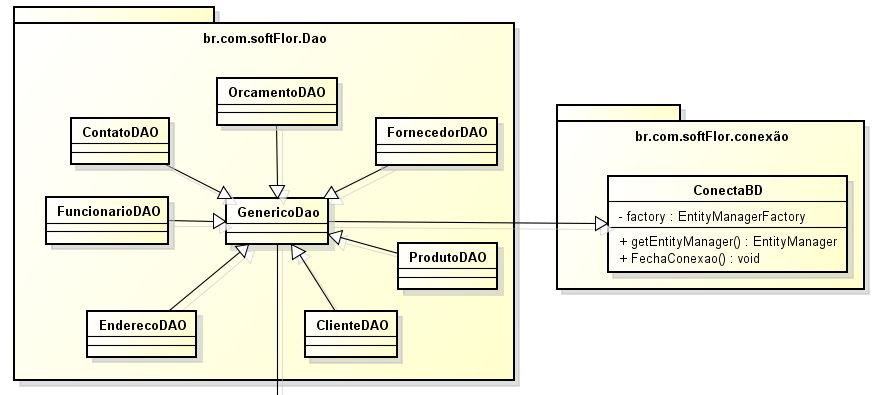
\includegraphics[width=14cm]{imagens/diagramas/Classes02}
\fonte{Autor próprio}
\label{fig:Diagrama de classes 01}
\end{figure}

\begin{figure}[H]
\centering
\caption{Diagrama de classes - Parte 02}
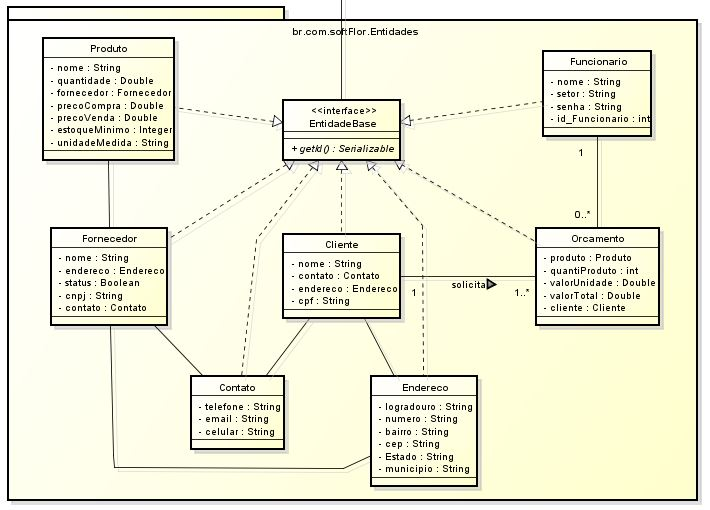
\includegraphics[width=16cm]{imagens/diagramas/Classes01}
\fonte{Autor próprio}
\label{fig:Diagrama de classes 02}
\end{figure}

	
\chapter{Diagramas de atividade}

\begin{figure}[h]
\centering
\caption{Diagrama de atividade - Cadastrar produto}
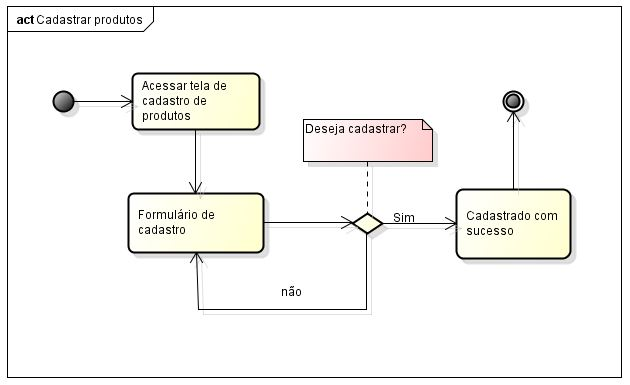
\includegraphics[width=12cm]{imagens/diagramas/atCadastrar}
\fonte{Autor próprio}
\label{fig:Diagrama de atividade - Cadastrar}
\end{figure}


\begin{figure}[h]
\centering
\caption{Diagrama de atividade - Editar produto}
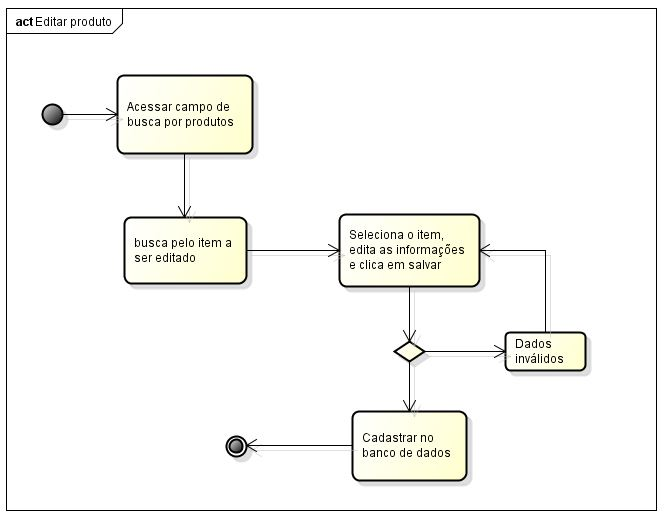
\includegraphics[width=12cm]{imagens/diagramas/atEditar}
\fonte{Autor próprio}
\label{fig:Diagrama de sequência - Editar}
\end{figure}

\begin{figure}[H]
\centering
\caption{Diagrama de atividade - Excluir produto}
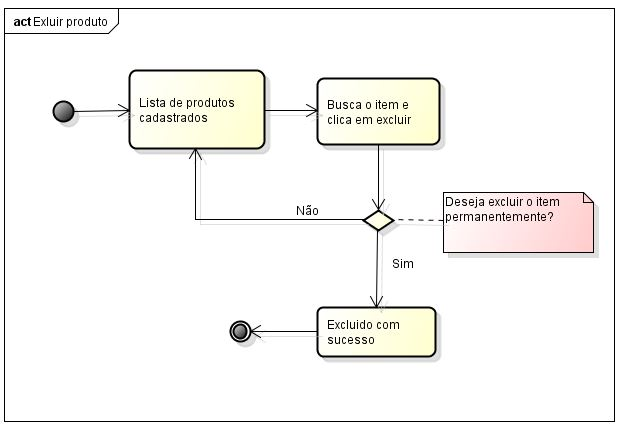
\includegraphics[width=12cm]{imagens/diagramas/atExcluir}
\fonte{Autor próprio}
\label{fig:Diagrama de sequência - Excluir}
\end{figure}



	
\chapter{Diagramas de sequência}

\begin{figure}[h]
\centering
\caption{Diagrama de sequência - Cadastrar produto}
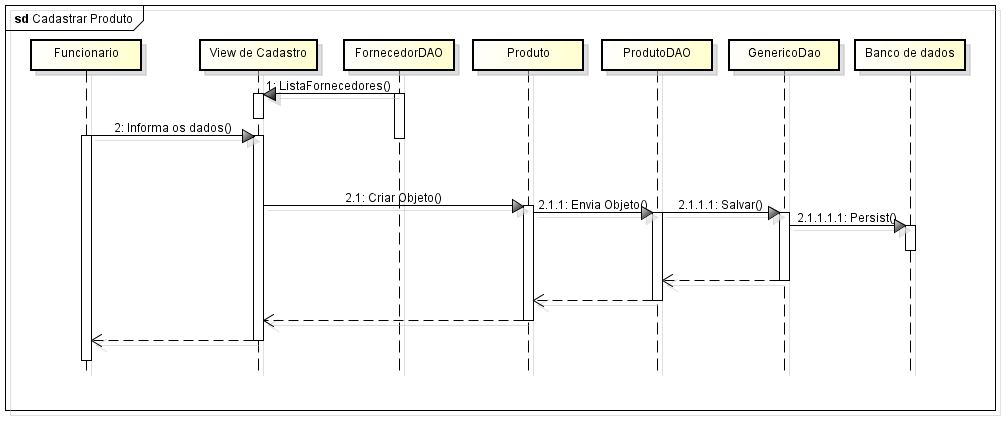
\includegraphics[width=15cm]{imagens/diagramas/sequCadastrar}
\fonte{Autor próprio}
\label{fig:Diagrama de sequência - Excluir}
\end{figure}

\begin{figure}[H]
\centering
\caption{Diagrama de sequência - Editar produto}
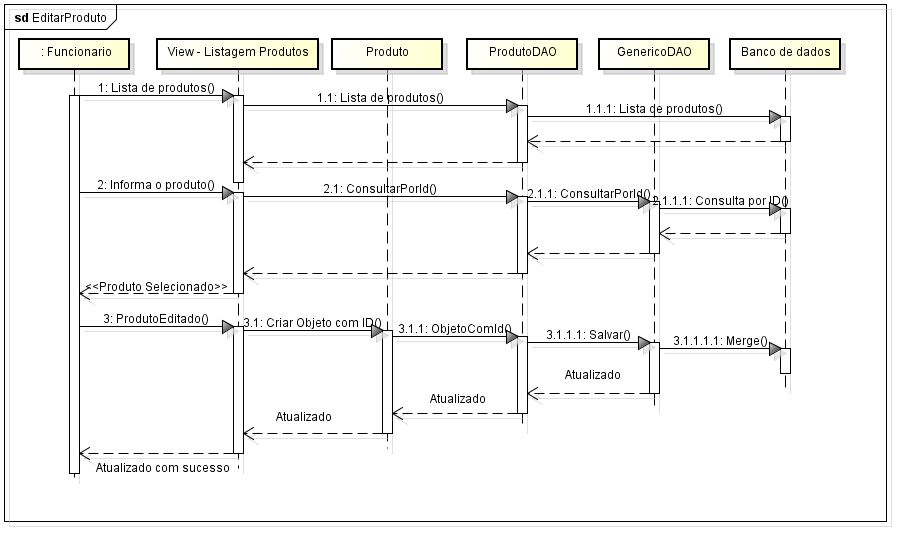
\includegraphics[width=14cm]{imagens/diagramas/sequEditar}
\fonte{Autor próprio}
\label{fig:Diagrama de sequência - Excluir}
\end{figure}

\begin{figure}[H]
\centering
\caption{Diagrama de sequência - Excluir produto}
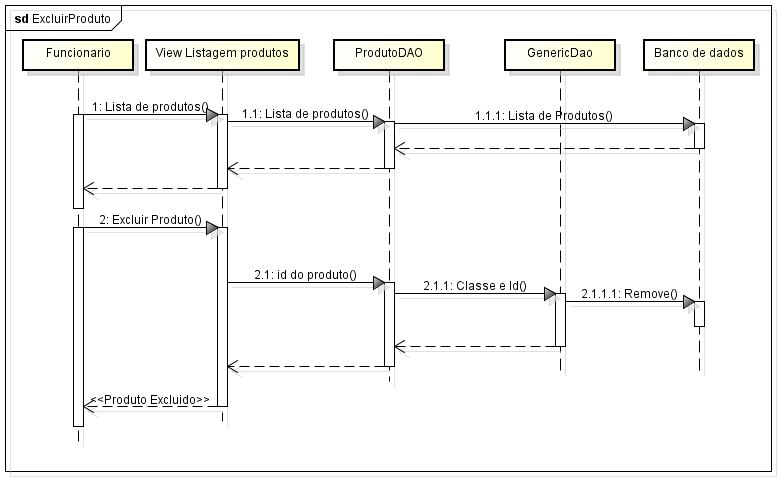
\includegraphics[width=14cm]{imagens/diagramas/sequExcluir}
\fonte{Autor próprio}
\label{fig:Diagrama de sequência - Excluir}
\end{figure}


\chapter{Diagrama MER}
\begin{figure}[h]
\centering
\caption{Diagrama MER}
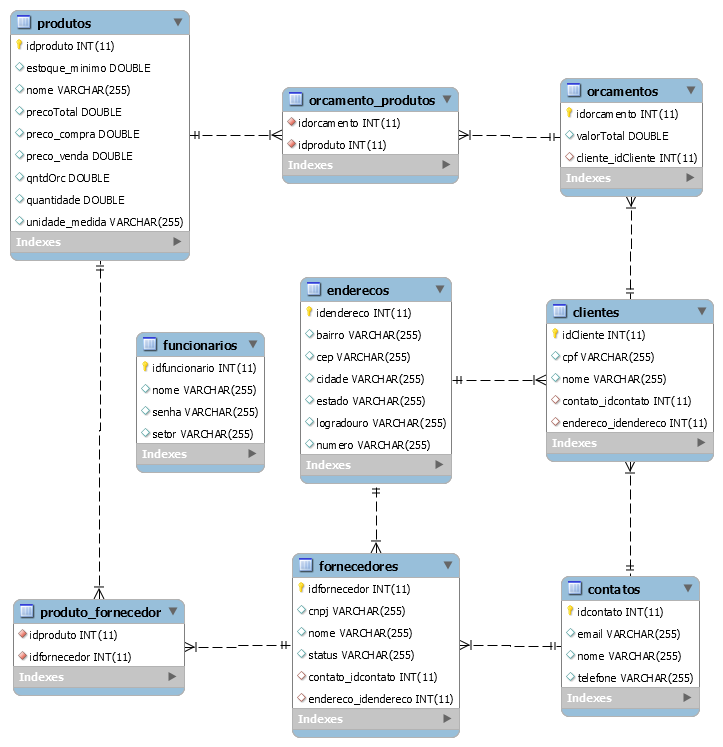
\includegraphics[width=16cm]{imagens/diagramas/bd2}
\fonte{Autor próprio}
\label{fig:Diagrama MER}
\end{figure}

\chapter{Código Java e Código do Banco de dados}
	% ---
	Todos os códigos deste sistema estão disponíveis na plataforma de hospedagem de código-fonte GitHub através do endereço: \url{https://github.com/loardjulio/SoftFlor.git}
	
\end{anexosenv}


% 05: Índices
%%---------------------------------------------------------------------
% INDICE REMISSIVO
%---------------------------------------------------------------------
\phantompart
\printindex
%---------------------------------------------------------------------


% Capa do CD (opcional)
%\input{pos-textual/capa-cd}